\documentclass[informe.tex]{subfiles}
\begin{document}

%\chapter{Introducción}

\justify

La función de red es la transformada de Laplace de la respuesta al impulso. Su forma es una razón
de dos polinomios de la frecuencia complejas.

Una función de red $F(s)$ puede ser \newline
- Una función propia de impedancia o admitancia de un elemento de un puerto. \newline
- Una función de transferencia entre el puerto de entrada y el puerto de salida de una red de dos puertos

Es una función racional con coeficientes reales

\begin{equation}
F(s) = \frac{A(s)}{B(s)}
     = \frac{ \sum_{i=0}^{m} a_i \cdot s^{i}} 
            {\sum_{i=0}^{n} b_i \cdot s^{i}}
     = \frac{ M_1(s)+N_1(s) }{ M_2(s)+N_2(s) }
\end{equation}


Donde el numerado y el denominador son dos polinomios complejos.

\begin{equation}
M(j \omega ) = Re[F(j \omega) ] 
\end{equation} y
\begin{equation}
N(j \omega ) = Im[F(j \omega) ] 
\end{equation} 


\textbf{Funciones real positiva y pasividad}


Se puede caracterizar un elemento de un dispositivo de un puerto, en condiciones iniciales nulas, sin fuentes independientes por las funciones de admitancia o de impedancia.

Cada función real positiva se puede realizar como una una función propia de una red que contiene solo elementos RLC positivos, transformadores ideales, bobinas acopladas, etc.\newline


\textbf{Función real positiva}
Es real positiva si:
1- $F(s)$ es real cuando $s$ es real. Exige que todos los coeficientes sean reales.
2- $Real{F(s)}>=0$ para $Real{s}>=0$.\newline

Entonces una función real positiva se puede realizar como una función de impedancia o de admitancia de un dispositivo de un puerto solo con elementos pasivos.\newline

\textbf{Teorema}\newline
La función de impedancia o admitancia de una red de un puerto es una función real positiva 

\textbf{Demostración}
Se demuestra con con el teorema de tellenge

\begin{figure}[h]
		\centering
		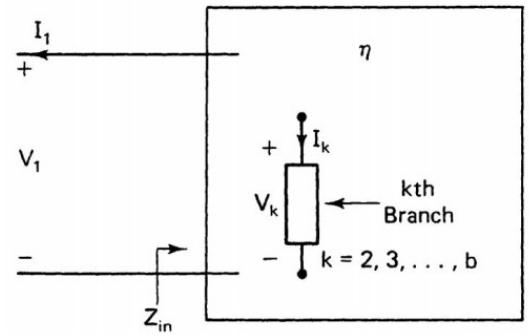
\includegraphics[scale=0.8]{tellenge.png}
		\caption{Representación de una red de un puerto}
		\label{fig:realizacion_de_redes:intro:tellenge}
		\end{figure}	



\end{document}	
